\documentclass{amsart}
\usepackage[usefamily=sage]{pythontex}
\usepackage[utf8]{inputenc}
\usepackage{tikz}

\newtheorem{thm}{Teorema}
\newtheorem{ejer}[thm]{Ejercicio}
\newtheorem{defn}[thm]{Definición}
\newtheorem{ejem}[thm]{Ejemplo}
\newtheorem{lem}[thm]{Lema}

\title{Tarea 07. Grafos}
\author{Manuel Bernal Hernández}

\begin{document}
\maketitle

\begin{ejer}
Dado el siguiente grafo:


\begin{center}
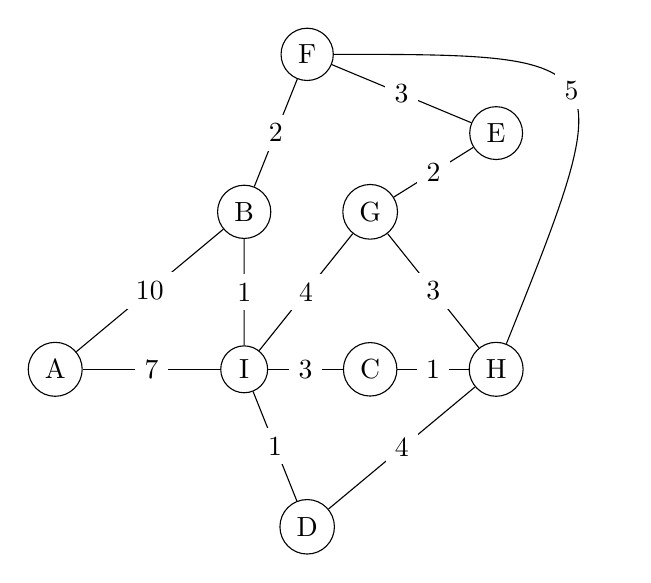
\begin{tikzpicture}[baseline=9mm,xscale = 0.8, vertice/.style = {fill=white,circle,draw}]
\node[vertice] (A) at (-1,1) {A};
\node[vertice] (B) at (2,3) {B};
\node[vertice] (C) at (4,1) {C};
\node[vertice] (D) at (3,-1) {D};
\node[vertice] (E) at (6,4) {E};
\node[vertice] (F) at (3,5) {F};
\node[vertice] (G) at (4,3) {G};
\node[vertice] (H) at (6,1) {H};
\node[vertice] (I) at (2,1) {I};

\draw (A) -- node[fill=white] {10} (B);
\draw (A) -- node[fill=white] {7} (I);
\draw (B) -- node[fill=white] {1} (I);
\draw (I) -- node[fill=white] {3} (C);
\draw (I) -- node[fill=white] {1} (D);
\draw (H) -- node[fill=white] {4} (D);
\draw (I) -- node[fill=white] {4} (G);
\draw (G) -- node[fill=white] {2} (E);
\draw (G) -- node[fill=white] {3} (H);
\draw (C) -- node[fill=white] {1} (H);
\draw (E) -- node[fill=white] {3} (F);
\draw (B) -- node[fill=white] {2} (F);
\draw (F) .. controls (8,5) .. node[fill=white] {5} (H);
\end{tikzpicture}
\end{center}
\end{ejer}

\begin{enumerate}
\item Calcula el árbol generador minimal del siguiente grafo usando el
algoritmo de Kruskal.
\item Calcula el árbol generador minimal del siguiente grafo usando el
algoritmo de Prim.
\end{enumerate}

{\it Solución:}

% Escribe tu solucion para el ejercicio
(1)
Ordenamos
1. Peso 1: CH, ID, BI
2. Peso 2: BF, GE
3. Peso 3: IC, FE, IC
4. Peso 4: IG, DH
5. Peso 5: FH
6. Peso 7: AI
7. Peso 10: AB

Colocamos las aristas de menor a mayor peso sin crear ciclos:
\begin{center}
    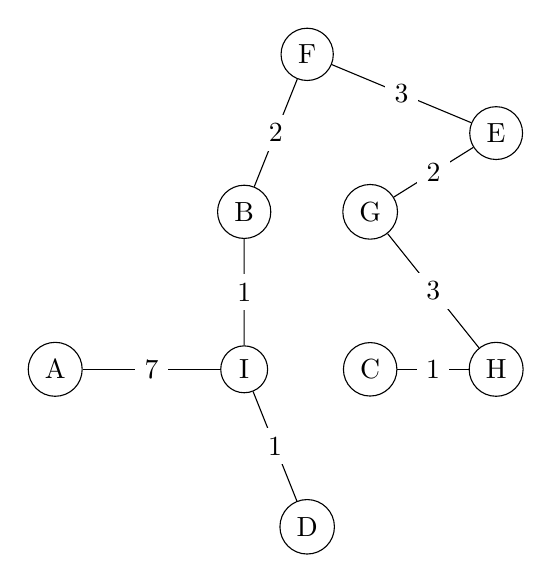
\begin{tikzpicture}[baseline=9mm, xscale=0.8, vertice/.style={fill=white, circle, draw}]
        \node[vertice] (A) at (-1, 1) {A};
        \node[vertice] (B) at (2, 3) {B};
        \node[vertice] (C) at (4, 1) {C};
        \node[vertice] (D) at (3, -1) {D};
        \node[vertice] (E) at (6, 4) {E};
        \node[vertice] (F) at (3, 5) {F};
        \node[vertice] (G) at (4, 3) {G};
        \node[vertice] (H) at (6, 1) {H};
        \node[vertice] (I) at (2, 1) {I};
        
        \draw (A) -- node[fill=white] {7} (I);
        \draw (B) -- node[fill=white] {1} (I);
        \draw (I) -- node[fill=white] {1} (D);
        \draw (G) -- node[fill=white] {2} (E);
        \draw (G) -- node[fill=white] {3} (H);
        \draw (C) -- node[fill=white] {1} (H);
        \draw (E) -- node[fill=white] {3} (F);
        \draw (B) -- node[fill=white] {2} (F);
    \end{tikzpicture}
\end{center}

(2)
Para el algoritmo de Prim, empezamos pintando el nodo $I$ de verde, y pintando los nodos de conectan las aristas de menor a mayor coste hasta terminar sin ciclos:
\begin{center}
    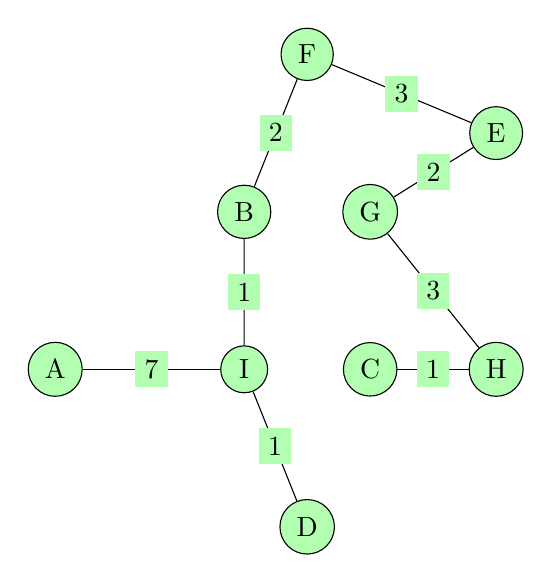
\begin{tikzpicture}[baseline=9mm, xscale=0.8, verde/.style={fill=green!30, circle, draw}]
        \node[verde] (A) at (-1, 1) {A};
        \node[verde] (B) at (2, 3) {B};
        \node[verde] (C) at (4, 1) {C};
        \node[verde] (D) at (3, -1) {D};
        \node[verde] (E) at (6, 4) {E};
        \node[verde] (F) at (3, 5) {F};
        \node[verde] (G) at (4, 3) {G};
        \node[verde] (H) at (6, 1) {H};
        \node[verde] (I) at (2, 1) {I};
        
        \draw (A) -- node[fill=green!30] {7} (I);
        \draw (B) -- node[fill=green!30] {1} (I);
        \draw (I) -- node[fill=green!30] {1} (D);
        \draw (G) -- node[fill=green!30] {2} (E);
        \draw (G) -- node[fill=green!30] {3} (H);
        \draw (C) -- node[fill=green!30] {1} (H);
        \draw (E) -- node[fill=green!30] {3} (F);
        \draw (B) -- node[fill=green!30] {2} (F);
    \end{tikzpicture}
\end{center}



% Fin del ejercicio

\end{document}


